%% LyX 2.0.2 created this file.  For more info, see http://www.lyx.org/.
%% Do not edit unless you really know what you are doing.
\documentclass[english]{article}
\usepackage[OT1]{fontenc}
\usepackage[latin9]{inputenc}
\usepackage{geometry}
\geometry{verbose,tmargin=2.5cm,bmargin=2.5cm,lmargin=2.5cm,rmargin=2.5cm}
\usepackage{float}
\usepackage{graphicx}
\usepackage{babel}

\usepackage{tikz}
\usepackage{pgfplots}
\usepackage{circuitikz}
\usetikzlibrary{arrows, positioning, calc,shapes}

\begin{document}

\title{Design of digital integrated systems: optimisation of a 16 bit Brent-Kung
adder}


\author{Your name here}

\maketitle

\section{Schematic and optimisation}


\subsection{Optimisation}

On this page you describe the optimisations you have used
\begin{itemize}
\item Architectural

\begin{itemize}
\item We changed this gate

\begin{itemize}
\item like this
\item and like this
\item and like this
\end{itemize}
\item The main effects are

\begin{itemize}
\item this 
\item and this
\end{itemize}
\end{itemize}
\item Sizing

\begin{itemize}
\item we increased the size of 

\begin{itemize}
\item this transistor
\item and this transistor
\item etc.
\end{itemize}
\end{itemize}
\end{itemize}
All in all you should have about two pages of explication (including
the header).

\section{Results}
Please fill in table \ref{table1}. Additional columns may be added, but provide at 
least one column with the data for the point with delay 650 ps.

\begin{table}[b]
\centering
\begin{tabular}{ |l|r| }
\hline
Delay & 650 ps \\
Supply & x.xx V \\
Switching Energy & xxx fJ \\
DC power & x.xx nW \\ 
\hline
\end{tabular}
\caption{Final performance of the circuit}
\label{table1}
\end{table}

\newpage{}


\subsection{Schematic}

\begin{figure}[H]
\begin{centering}
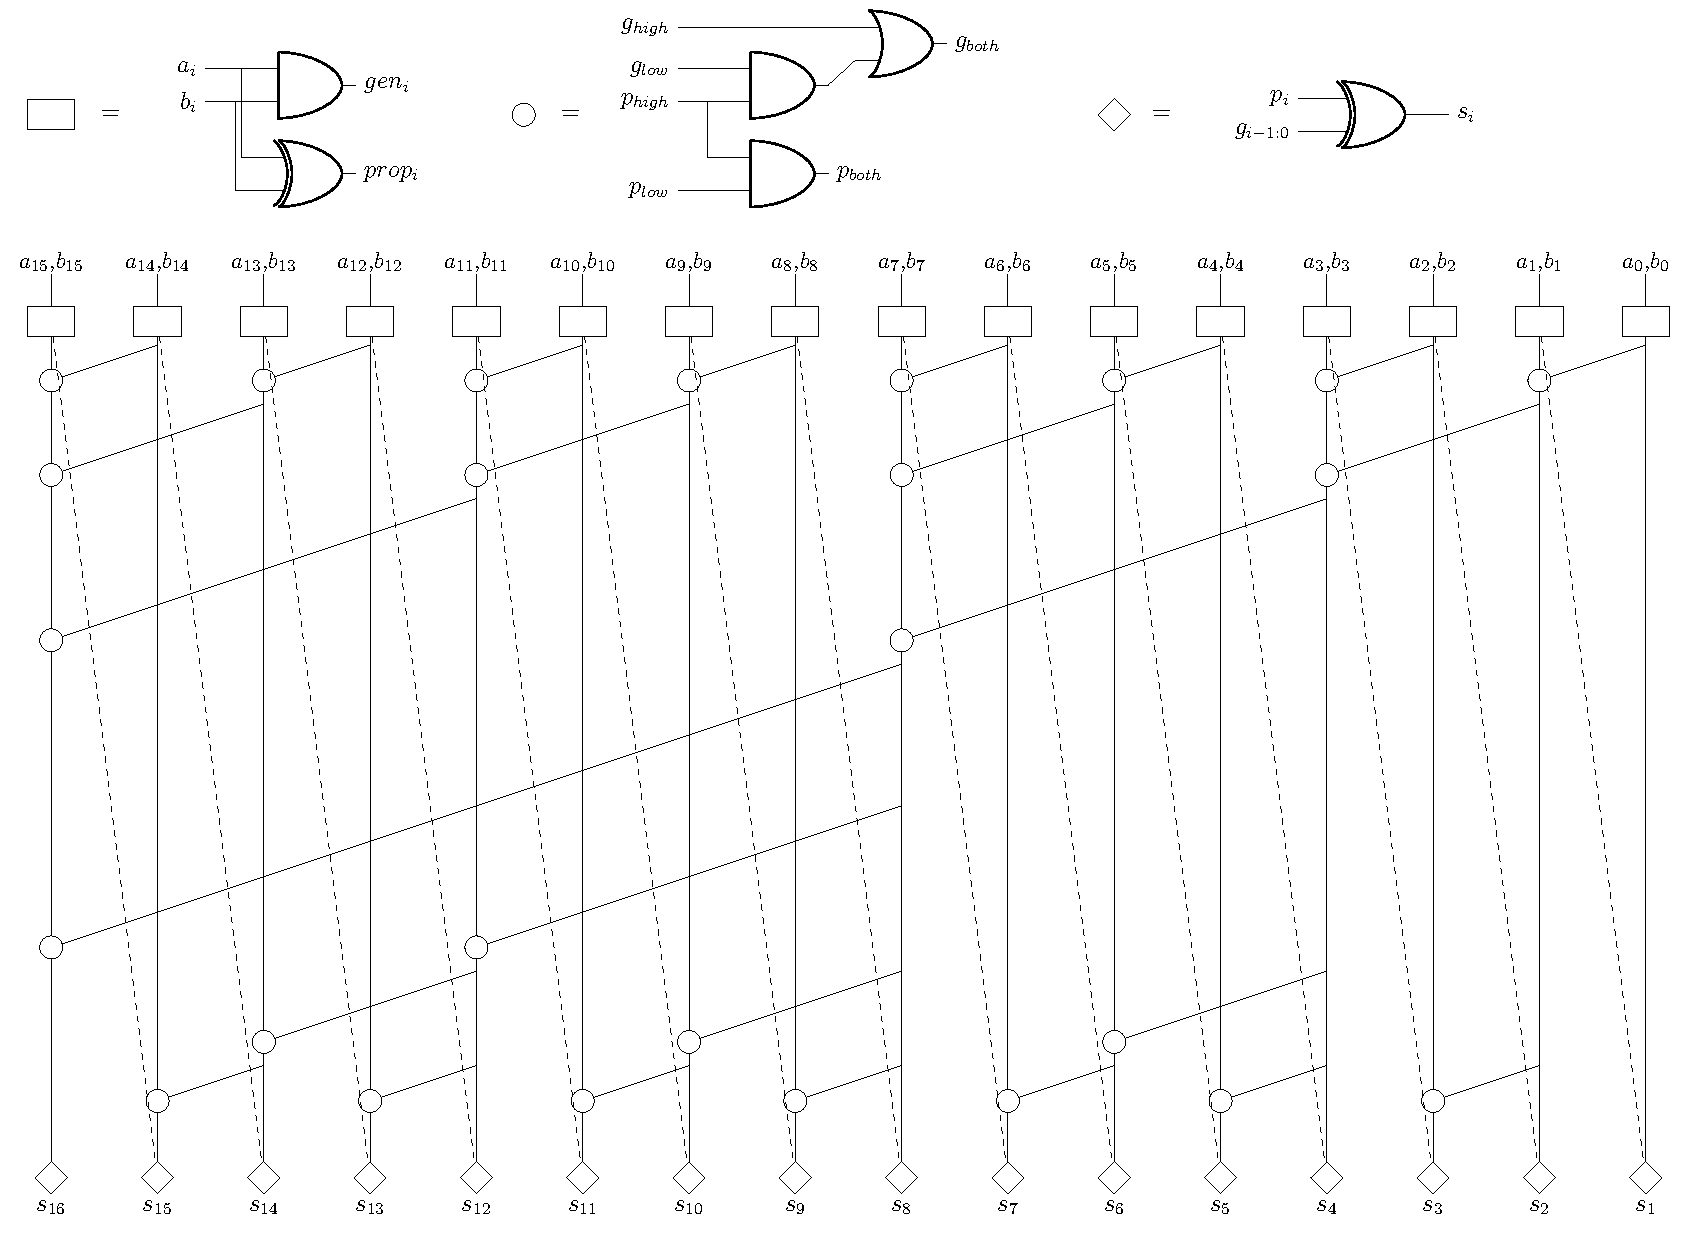
\includegraphics[angle=90,width=0.9\textwidth]{figures/Brent-Kung_tex}
\par\end{centering}
\caption{Schematic of the optimised adder}
\end{figure}





\end{document}
